\chapter{Experiment and Application Design}




This chapter describes the design of the experiment framework, both the experiment and the application side. The application will be explained from the system design point-of-view and the user experience perspective. First, The application high-level decision and work flow are explained using use case diagram. Then, the application system is describe more detail using flow chart and class diagram.



\section{Experiment Design}
\subsection{Participant}
21 Participants are participated in the study. All of the participant are student of University of Edinburgh. 3 students participate as a tester to ensure the application works perfectly. While 18 students conduct the experiment, and their data are analyzed.

\subsection{Procedure}
The experiment is conducted as a form of quiz where a number of questions is presented to the participant and the participant need to look the answer in the answer page. During the question and answer task there will be notification showed up. The participant can click the notification, and the android phone will get redirected to another application. After all, the participant can go back to the experiment application again.

During these experiment, three studies will be conducted. On every study 10 questions with the same category will be presented to the participant. The study is conducted using a silent lab room in a forrest hill lab and meeting room on the library. The room is keep empty and quite to keep the participant from any distraction.
These studies are explained below :
\begin{itemize}
\item study 1 : one question at a time will be presented to 4 participants.
\item study 2 : one or two questions at a time will be presented to 11 participants.
\item study 3 : one question is presented to 3 participants. on each time a participant look at the question they required to change the room. The participant is instructed to walk outside the room to the corridor or come back to the room.
\end{itemize}
\subsection{Goal}
The purpose of the experiment is to analyze how people lost their intention on the event boundary and what is the effect of multiple intention of the failure of prospective memory.

\subsection{Question}
During the experiment 10 questions is used. The question is designed as simple as possible so it does not require the participant to remember long context of the question. The particular question and answer page is chosen so that the participant should read carefully to find the answer.
The questions, link to the answer and its answer are listed on the table \ref{tab:questions}

% \begin{table}[!h]
%   \centering
% \begin{longtable}{|p{0.5cm}|p{4.5cm}|p{7cm}|p{3cm}|  }
%  \hline
%  No& Question & Answer link & Asnwer \\
%  \hline
%  1 & What is the original name of the titanic movie ?  & https://www.simplemost.com/15-fun-facts-probably-didnt-know-titanic/ & Planet ice\\
%  2 & In the movie "Lord of the Rings", How tall is Gandalf ? & https://www.phactual.com/14-fun-facts-about-the-lord-of-the-rings-the-fellowship-of-the-ring/ & Seven foot\\
%  3 & How many actors played both in Game of Thrones and in the Harry Potter movies ? & http://screenrant.com/best-facts-game-of-thrones-trivia/ & 9\\
%  4 & What is the meaning of Dumbledore in the Harry Potter movies ? & http://www.teenvogue.com/gallery/harry-potter-facts & Bumbelbee \\
%  5 & How many years has “How i met your mother” been filmed ? & https://www.phactual.com/10-fun-facts-about-how-i-met-your-mother/ & 9 years \\
%  6 &  How many baloons are attached to carl’s house in the "UP" movie ? & https://filmschoolrejects.com/10-fun-facts-about-pixars-up-1749a61575ca/ & 10,297 \\
%  7 & Where does marvel get the idea of the black spiderman suit ? & http://screenrant.com/best-marvel-facts-trivia-movies-tv-comics-superheroes/ & Fan or Randy \\
%  8 & What is the most expensive movie of all time ? & https://www.factretriever.com/hollywood-movies-facts & Avatar\\
%  9 & How many academy awards has the movie "UP" been nominated to ? &  http://www.imdb.com/title/tt1049413/trivia & two \\
% 10 & What is the most watched episode on the show “How i met your mother” ? & https://ritely.com/how-i-met-your-mother-trivia/ & The finale episode \\
%    \hline
% \end{longtable}
%  \caption{The questions used in the experiment}
%  \label{tab:questions}
% \end{table}

\begin{table}[]
\centering
\small
\footnotesize
\setlength\tabcolsep{2pt}
\begin{tabu}to \textwidth {|X[0.5,l]|
							X[5,l]|
                            X[7,l]|
                            X[2.8,l]|}
\hline
No & Question                                                                        & Answer Link                                                                                   & Answer             \\ \hline
1  & What is the original name of the titanic movie ?                                & https://www.simplemost.com/15-fun-facts-probably-didnt-know-titanic/                          & Planet             \\ \hline
2  & In the movie "Lord of the Rings", How tall is Gandalf ?                         & https://www.phactual.com/14-fun-facts-about-the-lord-of-the-rings-the-fellowship-of-the-ring/ & Seven foot         \\ \hline
3  & How many actors played both in Game of Thrones and in the Harry Potter movies ? & http://screenrant.com/best-facts-game-of-thrones-trivia/                                      & 9                  \\ \hline
4  & What is the meaning of Dumbledore in the Harry Potter movies ?                  & http://www.teenvogue.com/gallery/harry-potter-facts                                           & Bumbelbee          \\ \hline
5  & How many years has “How i met your mother” been filmed ?                        & https://www.phactual.com/10-fun-facts-about-how-i-met-your-mother/                            & 9 years            \\ \hline
6  & How many baloons are attached to carl’s house in the "UP" movie ?               & https://filmschoolrejects.com/10-fun-facts-about-pixars-up-1749a61575ca/                      & 10,297             \\ \hline
7  & Where does marvel get the idea of the black spiderman suit ?                    & http://screenrant.com/best-marvel-facts-trivia-movies-tv-comics-superheroes/                  & Fan or Randy       \\ \hline
8  & What is the most expensive movie of all time ?                                  & https://www.factretriever.com/hollywood-movies-facts                                          & Avatar             \\ \hline
9  & How many academy awards has the movie "UP" been nominated to ?                  & http://www.imdb.com/title/tt1049413/trivia                                                    & two                \\ \hline
10 & What is the most watched episode on the show “How i met your mother” ?          & https://ritely.com/how-i-met-your-mother-trivia/                                              & The finale episode \\ \hline
\end{tabu}
 \caption{The questions used in the experiment}
 \label{tab:questions}
\end{table}


\subsection{Demographic question}
The participant answer demographic question on the end of the experiment.
the list of the demographic question can be seen on the Table \ref{tab:demographicQuestion}

\begin{table}[!h]
  \centering
\begin{longtable}{ |p{0.5cm}|>{\hspace{0pt}}p{5.5cm}|p{7cm}  }
 \hline
 No& Question & Answer options \\
 \hline
 1 & Often people go into a room to do something.  Though they know they intended to do something,they lose track of what they wanted to do. This same sort of thing can happen when using a smart phone, as well.  During the study, you may have clicked on a link, gone to the website, and then forgot what you intended to look up.  Did that happen to you at all during this study?  & Yes, No\\
 2 & During this study, did you ever look up an answer, then forget the answer before you were able to type it in? & Yes, No\\
 3 & During the course of this study, how many cell phone notifications did you receive ?' & 0,1,2,3 or more\\
 4 & How many notifications did you decide to click ? & 0,1,2,3 or more \\
 5 & As you were looking up information, did you ever follow a link you didn\'t need to follow, just out of interest ? & Yes,No \\
 6 &  During the study, did you read about or learn any new facts that were not answers to questions we asked ? & Yes, No \\
 7 & How old are you ? & - \\
 8 & What is your gender ? & -\\
 9 & What country are you come from ? &  - \\
10 & Is English your native language  & Yes,No\\
11 & How many years have you spoken English? If you are a native speaker please leave blank.  & -\\
11 & What kind of phone do you normally use ?  & non-smartphone, iphone, android, other\\
12 & How difficult did you find the smartphone in this study ?  & Very Hard, Hard, Average, Easy, Very Easy\\
12 & How frequently do you use a smartphone ?  & Don\'t own one, Daily, Weekly, Monthly\\

 \hline
\end{longtable}
 \caption{The demographic questions used in the experiment}
 \label{tab:demographicQuestion}
\end{table}

\subsection{Input Data}
The input data use in this experiment can be seen on \todo[inline]{put it inside the appendix}


\subsection{Consent form}
Consent form is a document to formally get the approval of the participant. By ensuring the participant understand the experiment. The participant will need to sign the document. The document can be seen on \todo[inline]{put in appendix}

\subsection{Participant information sheet}
The participant information is given to the participant before the experiment is conducted. it has the information about the experiment and the protection of the data produce during experiment. The participant information sheet can be seen on \todo[inline]{put inside an appendix}


\section{Android application and web server}

The framework is originally based on the \href{https://pennstate.qualtrics.com/jfe/form/SV_dpaKW6wlA1Fr7BX}
{web application} built by Prof. Alan Carlson and his team. The experiment framework is made extendable, dynamic and produceable so that other researcher can design and conduct various type of experiment using a high number of sample during the study of prospective memory.
 The Experiment framework consist of android application and web server application. The web server is used to upload the input file, set extra properties, and download the output data of the experiment , and the android application is used to conduct the experiment, track variables, and produce output data. The relation between these two component can be seen in figure \ref{fig:mainline}

\begin{figure}[h]
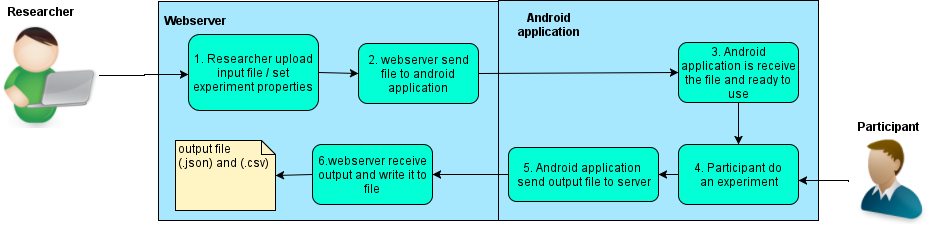
\includegraphics[scale=0.4]{framework_process}
\caption{mainline of the framework}
\label{fig:mainline}
\end{figure}

Researcher will need to start the webserver and use it to upload the input file of json format. the input file will get uploaded into the android application.  On the android application the researcher can set the experiment properties for example which experiment to conduct, the name of current participant etc. This is made because by using one input file the researcher can conduct multiple experiment with multiple participant without uploading the input file again, more of this feature will be discussed on the next implementation chapter. Furthermore, The application is able to track a group of variables of the participant during the experiment process. All the tracked variable and the mechanism of tracking will be discussed on the Tracker section. After finishing the experiment the output data inside the android application will be sent to the webserver which will be compiled to a json output file.

\section{Requirement}

The table \ref{tab:requirementList} below shows the list of all requirements of the application and its description.
% The main part are there are two
% main actors, a researcher and a participant. Researcher will able to set a input file and set parameters for the experiment. Participants then able to do the experiment by using the experiment application provided by the researcher. the application track the variables of the experiment. Finally, the researcher then able to download the experiment output\\

\begin{table}[!b]
  \centering
	\begin{tabular}{ |p{0.5cm}|p{5cm}|p{10cm}|  }
     \hline
     \multicolumn{3}{|c|}{Requirement List} \\
     \hline
     No& Name & Text \\
     \hline
     1   & Upload Input    & Researcher upload an .json input file to the application\\
     2 & Download Output & Researcher download a .json output file of the experiment\\
     3 & Set experiment properties & Researcher able to set extra experiment's properties apart from input file.
     \begin{itemize}
     \item study name
     \item participant Id
     \item researcher Id
     \item which experiment to conduct
     \end{itemize}\\
     4 & insert multiple category & Researcher insert multiple categories \\
     5 &  insert questions & On each category researcher insert multiple questions\\
     6 & set number of presented question & Researcher set how many question will be presented on each quiz phase   \\
     7 & set presented question behavior &  Researcher set whether the number of presented will be random each phase \\
     8 & insert post question  &  Researcher set whether the number of presented will be random each phase \\
       9 & insert notification  &  Researcher set notification with properties
    \begin{itemize}
    \item phase : which ordinal of the question will it be shown
    \item    activity : what activity will it be shown
    \item how many millisecond  it takes to wait before shown to the user
    \end{itemize}\\
      9 & see the questions  &  the participant can see the questions\\
      10 & show answer link and answer page &  the participant can clicked the answer links which will be  \\
      11 & fill the answer  &  the participant can answer by filling the answer box \\
      12 & show notification  &  the application can show and pop up notification \\
      13 & Track variables  &  The application can tracked/logged variables\\
    \hline
    \end{tabular}
 \caption{List of requirements}
 \label{tab:requirementList}
\end{table}

\section{Application Design}
The design of the entities, it's relationship, and the mechanism of the experiment will be discussed in this chapter. The design is based on the requirement describe earlier.

\subsection{Input and output}


The researcher needs to upload the input file that consist of all the experiment properties, and after the experiment done the result can be downloaded as a json file.
Json (Java Script object notation) is used as an input and output format because it is very easy for a human to read and write, also for the machine to parse and generate. Most of the current programming language and analysis software support json format. The json format consist of key and value pairs, on many language it is similar to dictionary, table or struct. This input file will then be uploaded and compiled to the android application.
Here is a simple example of the json format


\noindent\fbox{%
    \parbox{\textwidth}{%
       \{\\
    \hspace{10mm}    name :"John",\\
   \hspace{10mm}     age:21,\\
    \hspace{10mm}    hooby:swimming\\
       \}
       }
    }%

The table \ref{tab:inputFile} shows all the field for the input and its description. The output of the application will be a json file that consist of the experiment result which consist of the answer of the all the questions and tracked variables.
Example of the input and output are shown in the
appendix, show the input and output
:\todo[inline]{include the input and output example in appendix}
\begin{table}[!h]
  \centering
\begin{longtable}{ |p{0.5cm}|>{\hspace{0pt}}p{5.5cm}|p{1.6cm}|p{7cm}|  }
 \hline
 \multicolumn{4}{|c|}{Input} \\
 \hline
 No& Name & Type & Description \\
 \hline
 1 & Study.PreText  & String & a html string that will be shown at first on the experiment\\
 2 & Study.PostText & String & a html string that will be shown after the pretext\\
 3 & Study.NumExp & Integer & Researcher able to set extra experiment's properties apart from input file.\\
 4 & Study.Name &  String & The name of the study \\
 4 & Study.Id & String & Researcher insert multiple categories (Optional) \\
 5 &  Experiment.Name & String & The name of the experiment \\
 6 & Experiment.NumQuestion & Integer & Researcher set how many question will be presented on each quiz phase   \\
 7 & Experiment.MaxPresentedQuestion  & Integer &  Researcher set whether the number of presented will be change randomly in each phase \\
 8 & Experiment.RandomPresentedQuestion & Boolean &  Researcher set whether the number of presented will be random each phase \\
9 & Category.Id  & String &  Id of the category (Optional) \\
10 & Category.Name  & String & The name of the category \\
11 & Category.TotalQuestion & Integer  & The total size of the question on this category  \\
   12 & Category.QuestionOrder  &  String &  the order of how the question will be pulled from the list of question. "LINEAR" it will be pulled based on the input order, "RANDOM" it will be pulled randomly\\
   13 & Category.Question.Id  &  String & the unique Id of the question \\
   14 & Category.Question.Text  & String &  The question text \\
   15 & Category.Question.linkAnswer  &  String & the http/https  link of answer \\
   16 & Category.Question.Answer  & String & the answer of the question \\
     17 & Notification.App  & String & What application the phone will open if the participant click the notification \\
   18 & Notification.shift & Int &
   The number of phase when the notification should be shown. This will be explained more on the Notification section \\
   19 & Notification.Phase  & String & The activies name when the notification should be appeared\\
  20 & Notification.TimeToShow & Integer  &  how millisecond the application should wait before showing the notification \\
   21 & Notification.Url  &  String & what url or id the application will open if the participant clicked the notification \\
   22 & Notification.TitleText  & String & The title of the notification \\
   23 & Notification.MsgText  &  String & The text of the notification  \\
   \hline
\end{longtable}
 \caption{Explanation of the entities inside the input file}
 \label{tab:inputFile}
\end{table}


\subsection{Application entities}
The input file that the researcher uploaded will be generated to an object. The architecture of the object can be seen in the figure \ref{fig:Experiment_objects} . Each box represent an object that consist of properties and methods. The biggest object is a Study object, this object is acted as a container for other objects.

it works like a main bone of the application that hold another object e.g experiment and category. and also control the flow of the experiment. The arrow in the figure show the pointer on which particular experiment, category, questions and notification will be presented during the experiment. The study container also act as a tracker of some variables during the experiment.


The experiment object consist of properties on how the experiment will works, e.g experiment name, number of question will be asked, and how the question will be presented.
And the category object consist of multiple questions objects which consist of the question text and its answer link. Lastly, The notification consist of the parameter on when it will be shown on the experiment.

The Researcher will able to choose which experiment will be used and which notification will appeared and the participant can choose which category they want to answered. this selected experiment and category objects will be linked by study container and compiled as active category and active experiment, this will be explained much further on the implementation chapter.

\begin{figure}[!h]
\begin{center}
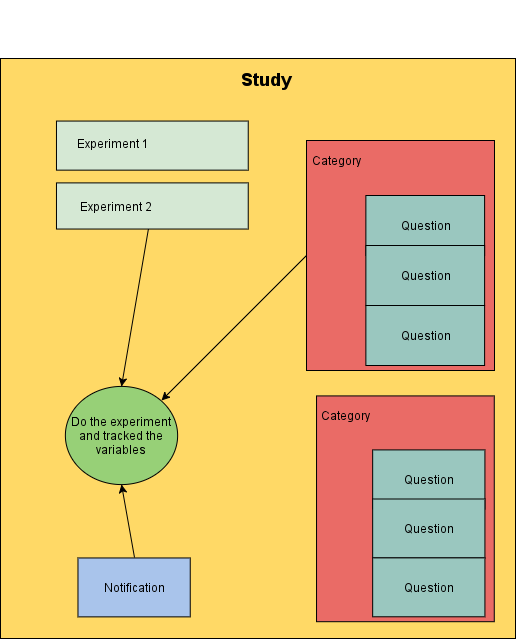
\includegraphics[scale=0.4]{quiz_Diagram}
\end{center}
\caption{Structure of the object inside the application}
\label{fig:Experiment_objects}
\end{figure}


\subsection{Application flow}


To make it easy to differentiate the experiment flow during the quiz (question and answering), the activity is divided into three parts question, answer and fill answer Activity.


\begin{figure}[!b]
\begin{center}
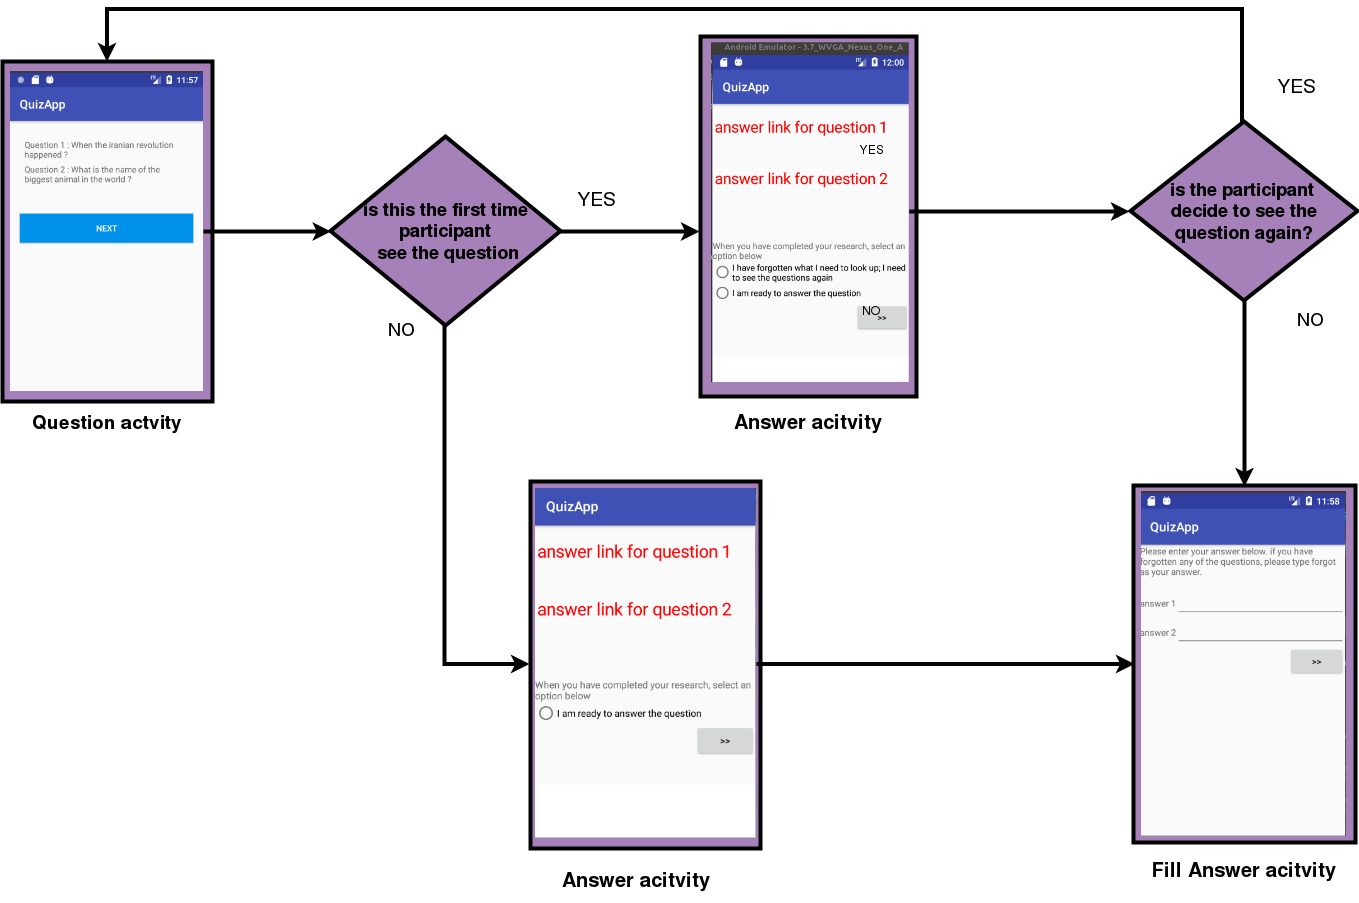
\includegraphics[scale=0.35]{Quiz_flow}
\end{center}
\caption{Quiz activity flow}
\label{fig:quiz_flow}
\end{figure}

Figure \ref{fig:quiz_flow} shows how the application will looks like and the flow of activities of the quiz. Based on the flow of quiz activity, the application should have properties describe on the table \ref{tab:requirementList}. these properties will be used to identify the status of the activity during the experiment.
% \begin{itemize}
% \item \textit{Shift} : This variable is used to count how many question-answer had been done.
% \item \textit{Phase} : this variable has a value on what activity is currently active on the application
% \item \textit{Active Category} : The active category that will be choose by the participant during the experiment. This category will contain list of questions.
% \item \textit{Active Experiment} : This variable will contains the properties of the current experiment, this properties is set by the researcher from the application
% \item \textit{Number of presented question} : this variable value shows how many question are asked at one \textit{shift} of question-answer.
% \item \textit{Active Question }: the current question and it's answer link that is presented to the participant. This active question is picked from the question list inside the active category. the number of active question is based on \textit{number of presented question} variable.
% \end{itemize}

\begin{table}[!t]
  \centering
	\begin{tabular}{ |p{0.5cm}|p{5cm}|p{10cm}|  }
     No& Properties name & Description \\
     \hline
     1   & \textit{Shift} & This variable is used to count how many question-answer had been done.\\
     2 & \textit{Phase} & This variable has a value on what activity is currently active on the application\\
     4 & \textit{Active Category} & The active category that will be choose by the participant during the experiment. This category will contain list of questions. \\
     5 &  \textit{Active Experiment} & This variable will contains the properties of the current experiment, this properties is set by the researcher from the application\\
     6 & \textit{Number of presented question} & this variable value shows how many question are asked at one \textit{shift} of question-answer.
\textit{Active Question }: the current question and it's answer link that is presented to the participant. This active question is picked from the question list inside the active category. the number of active question is based on \textit{number of presented question} variable.\\
    \end{tabular}
 \caption{List of application entity for the quiz activity}
 \label{tab:requirementList}
\end{table}



To be more descriptive about the application flow, figure \ref{fig:quiz_flowchart} shows the flow of the quiz and the how the quiz properties is updated.
\begin{itemize}
\item \textbf{Initialization} : firstly a \textit{phase} is initialize. The application then check if the experiment is still going which mean there still questions need to be asked. The quiz is finished if all the question has been asked.

\item \textbf{Question activity} : Secondly, the number of presented question will change randomly or stay constant.
Then before the question is picked from the active category , and the questions are shown to the participant.
\item \textbf{Answer activity} : Thirdly, The links for the answer page are shown to the participant, the participant then click the link and find the answer. During this phase the participant has a chance to see the question again. The participant can also decide to answer the question directly.
\item \textbf{fill answer activity} is the activity when the participant need to write the answer of the question on the text box. After that, the \textit{phase} variable is increased and the application will check again if the experiment is still going on and continue to question activity or finish.
\end{itemize}

\begin{figure*}[!t]
\begin{multicols}{2}
    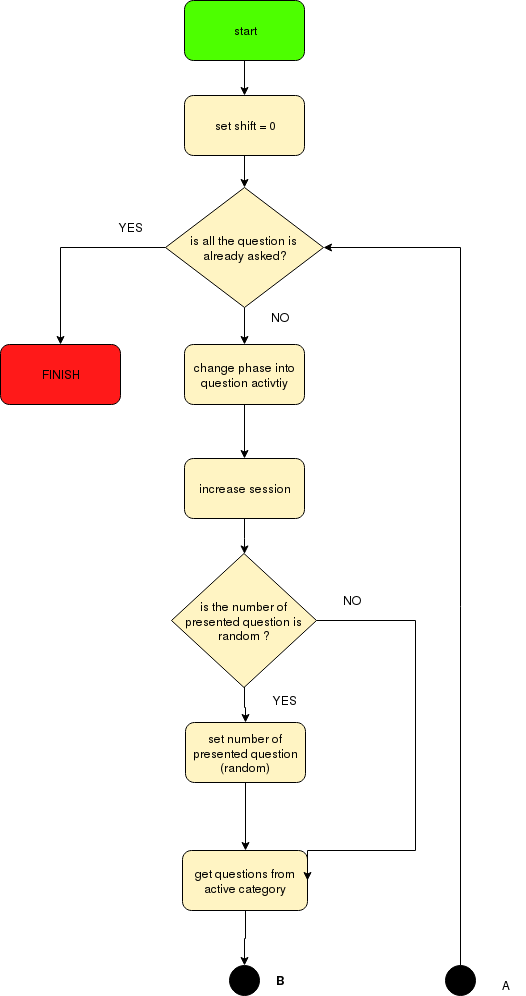
\includegraphics[scale=0.4]{Quiz_activity}\par
    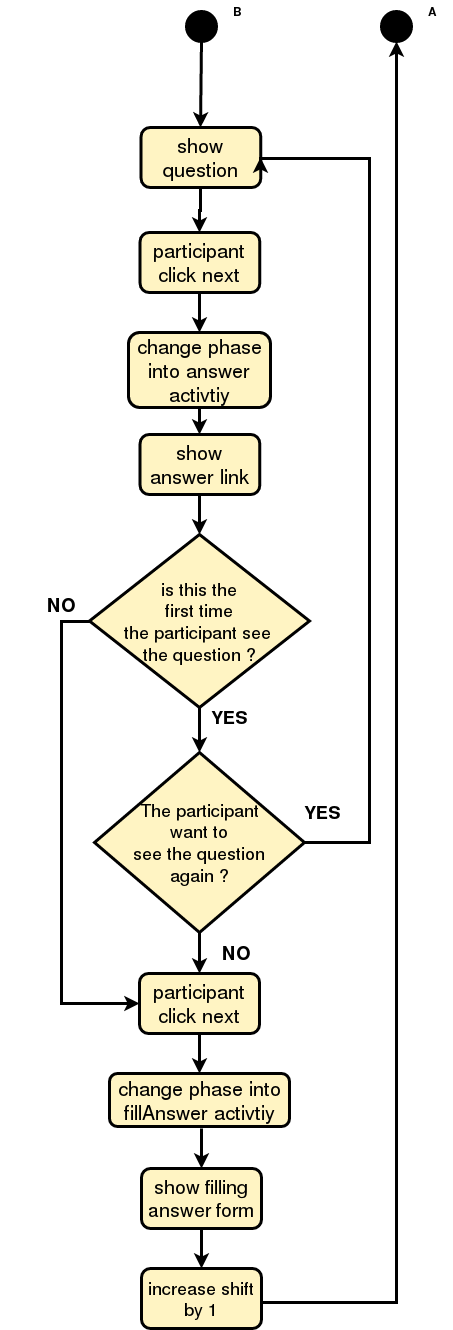
\includegraphics[scale=0.35]{Quiz_Activity_2}\par
    \end{multicols}
\caption{Quiz flowchart}
\label{fig:quiz_flowchart}
\end{figure*}



\subsection{Notification design}

Notification will be shown as a pop up box, as seen in figure \ref{fig:notification_flow}.
During the quiz activity the notification will be shown to the participant. If the participant click the notification then the phone will be redirected to another application.

The notification should have the following properties:
\begin{itemize}
\item \textit{shift} : this property is to decide on which shitft the notification will be shown, it will be compared to the \textit{shift} properties of the study object.
\item \textit{phase} : this properties is to decide on which activity (question, answer and fill answer) the notification will be shown.
\item \textit{app} : what application the notification will open, it also need to have a value of the user or url of the application.
\item \textit{timeToshow} : how millisecond the framework should wait before the notification will be shown
\item \textit{notification text} what is the message text inside the notification box
\end{itemize}
All of these parameters above can be set by the researcher from the input file.
\todo[inline]{make this as a table}

Figure \ref{fig:notification_flow} show the flow of the notification. The notification will be shown during the experiment process. If the user click the notification then the experiment application will be minimized and the android phone will be directed to another application. Then, the user can click the application icon to get back to the experiment application.

\begin{figure}
\begin{center}
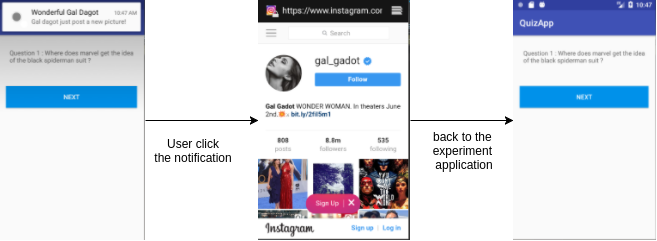
\includegraphics[scale=0.65]{notication}
\end{center}
\caption{Notification flow}
\label{fig:notification_flow}
\end{figure}



\subsection{tracked variable}
During the experiment the application should track variables. The following table consist of all the variables that the application track during the experiment. some of the variable has lb in front of their name, this mean that variable is tracked during the lookback process. A process when the participant look the question again for the second time.

\begin{table}
  \centering
\begin{longtable}{ |p{0.5cm}|p{4cm}|p{2.3cm}|p{6cm}|  }
 \hline
 \multicolumn{4}{|c|}{Tracked variables list} \\
 \hline
 No& Variable's name & Type & Description \\
 \hline
 1 & TTLQ & Long  & total time (in millisecond) when the participant to see the question then click next button\\
 2 & lb\_TTLQ & Long & similar with TTLQ and the participant decide to look the question again\\
 3 & LookBack & Boolean & True if the participant decide to look at the question again, false otherwise. \\
 4 & TTLB & Long & total time (in millisecond) when the participant see the answer links and decide to look the question again or answer the question (next button) \\
 5 & lb\_TTLB & Long & Similar with TTLB and the participant decide to look at the question again.Then, answer links are shown again to the participant\\
 6 & visited\_links & List of String & The list of links clicked/visited by the participant after clicking the answer links\\
 7 & time\_visited\_links & List of Long  & List of the total time (in millisecond) the participant stay on a page after clicking link\\
 8 & lb\_visited\_links & List of String & similar with visited\_links but the participant have decided to see the question again then return to the answer links window\\
 9 & lb\_time\_visited\_links & List of Long & Similar with time\_visited\_links but the participant decide to look at the question again then click the answer links\\
 10 & TTLA & Long & Total time (in millisecond) the participant see the fill answer window and then click next\\
 11 & TTLFA & Long & Total time (in milisecond) the participant write the answer on the text box\\
 12 &  num\_notif & Integer & how many notification is shown during the a question \\
 14 & TTLN & Long & Total time (in millisecond) it tooks the participant after clicking the notification to back to experiment application\\
\hline
\end{longtable}
\caption{variables need to be tracked}
 \label{tab:trackedVarible}
\end{table}
\par
